% GNUPLOT: LaTeX picture with Postscript
\begingroup
\newcommand{\ft}[0]{\footnotesize}\newcommand{\ty}[0]{\tiny}
  \makeatletter
  \providecommand\color[2][]{%
    \GenericError{(gnuplot) \space\space\space\@spaces}{%
      Package color not loaded in conjunction with
      terminal option `colourtext'%
    }{See the gnuplot documentation for explanation.%
    }{Either use 'blacktext' in gnuplot or load the package
      color.sty in LaTeX.}%
    \renewcommand\color[2][]{}%
  }%
  \providecommand\includegraphics[2][]{%
    \GenericError{(gnuplot) \space\space\space\@spaces}{%
      Package graphicx or graphics not loaded%
    }{See the gnuplot documentation for explanation.%
    }{The gnuplot epslatex terminal needs graphicx.sty or graphics.sty.}%
    \renewcommand\includegraphics[2][]{}%
  }%
  \providecommand\rotatebox[2]{#2}%
  \@ifundefined{ifGPcolor}{%
    \newif\ifGPcolor
    \GPcolortrue
  }{}%
  \@ifundefined{ifGPblacktext}{%
    \newif\ifGPblacktext
    \GPblacktextfalse
  }{}%
  % define a \g@addto@macro without @ in the name:
  \let\gplgaddtomacro\g@addto@macro
  % define empty templates for all commands taking text:
  \gdef\gplbacktext{}%
  \gdef\gplfronttext{}%
  \makeatother
  \ifGPblacktext
    % no textcolor at all
    \def\colorrgb#1{}%
    \def\colorgray#1{}%
  \else
    % gray or color?
    \ifGPcolor
      \def\colorrgb#1{\color[rgb]{#1}}%
      \def\colorgray#1{\color[gray]{#1}}%
      \expandafter\def\csname LTw\endcsname{\color{white}}%
      \expandafter\def\csname LTb\endcsname{\color{black}}%
      \expandafter\def\csname LTa\endcsname{\color{black}}%
      \expandafter\def\csname LT0\endcsname{\color[rgb]{1,0,0}}%
      \expandafter\def\csname LT1\endcsname{\color[rgb]{0,1,0}}%
      \expandafter\def\csname LT2\endcsname{\color[rgb]{0,0,1}}%
      \expandafter\def\csname LT3\endcsname{\color[rgb]{1,0,1}}%
      \expandafter\def\csname LT4\endcsname{\color[rgb]{0,1,1}}%
      \expandafter\def\csname LT5\endcsname{\color[rgb]{1,1,0}}%
      \expandafter\def\csname LT6\endcsname{\color[rgb]{0,0,0}}%
      \expandafter\def\csname LT7\endcsname{\color[rgb]{1,0.3,0}}%
      \expandafter\def\csname LT8\endcsname{\color[rgb]{0.5,0.5,0.5}}%
    \else
      % gray
      \def\colorrgb#1{\color{black}}%
      \def\colorgray#1{\color[gray]{#1}}%
      \expandafter\def\csname LTw\endcsname{\color{white}}%
      \expandafter\def\csname LTb\endcsname{\color{black}}%
      \expandafter\def\csname LTa\endcsname{\color{black}}%
      \expandafter\def\csname LT0\endcsname{\color{black}}%
      \expandafter\def\csname LT1\endcsname{\color{black}}%
      \expandafter\def\csname LT2\endcsname{\color{black}}%
      \expandafter\def\csname LT3\endcsname{\color{black}}%
      \expandafter\def\csname LT4\endcsname{\color{black}}%
      \expandafter\def\csname LT5\endcsname{\color{black}}%
      \expandafter\def\csname LT6\endcsname{\color{black}}%
      \expandafter\def\csname LT7\endcsname{\color{black}}%
      \expandafter\def\csname LT8\endcsname{\color{black}}%
    \fi
  \fi
    \setlength{\unitlength}{0.0500bp}%
    \ifx\gptboxheight\undefined%
      \newlength{\gptboxheight}%
      \newlength{\gptboxwidth}%
      \newsavebox{\gptboxtext}%
    \fi%
    \setlength{\fboxrule}{0.5pt}%
    \setlength{\fboxsep}{1pt}%
\begin{picture}(4030.00,4608.00)%
    \gplgaddtomacro\gplbacktext{%
      \csname LTb\endcsname%
      \put(528,638){\makebox(0,0)[r]{\strut{}\ft 0.2}}%
      \csname LTb\endcsname%
      \put(528,956){\makebox(0,0)[r]{\strut{}\ft 0.21}}%
      \csname LTb\endcsname%
      \put(528,1275){\makebox(0,0)[r]{\strut{}\ft 0.22}}%
      \csname LTb\endcsname%
      \put(528,1593){\makebox(0,0)[r]{\strut{}\ft 0.23}}%
      \csname LTb\endcsname%
      \put(528,1911){\makebox(0,0)[r]{\strut{}\ft 0.24}}%
      \csname LTb\endcsname%
      \put(528,2230){\makebox(0,0)[r]{\strut{}\ft 0.25}}%
      \csname LTb\endcsname%
      \put(528,2548){\makebox(0,0)[r]{\strut{}\ft 0.26}}%
      \csname LTb\endcsname%
      \put(528,2866){\makebox(0,0)[r]{\strut{}\ft 0.27}}%
      \csname LTb\endcsname%
      \put(528,3185){\makebox(0,0)[r]{\strut{}\ft 0.28}}%
      \csname LTb\endcsname%
      \put(528,3503){\makebox(0,0)[r]{\strut{}\ft 0.29}}%
      \put(660,418){\makebox(0,0){\strut{}\ft 0}}%
      \put(1778,418){\makebox(0,0){\strut{}\ft 0.1}}%
      \put(2897,418){\makebox(0,0){\strut{}\ft 0.2}}%
      \put(3121,418){\makebox(0,0){\strut{}}}%
      \put(3344,418){\makebox(0,0){\strut{}}}%
      \put(3568,418){\makebox(0,0){\strut{}\ft 0.5}}%
    }%
    \gplgaddtomacro\gplfronttext{%
      \csname LTb\endcsname%
      \put(-44,2070){\rotatebox{-270}{\makebox(0,0){\strut{}\ft Acceptance rate}}}%
      \put(2114,154){\makebox(0,0){\strut{}\ft Attack probabilities}}%
      \csname LTb\endcsname%
      \put(1547,4475){\makebox(0,0)[r]{\strut{}\ty UC-DOR}}%
      \csname LTb\endcsname%
      \put(1547,4335){\makebox(0,0)[r]{\strut{}\ty G2C3}}%
      \csname LTb\endcsname%
      \put(1547,4195){\makebox(0,0)[r]{\strut{}\ty G2C4}}%
      \csname LTb\endcsname%
      \put(1547,4055){\makebox(0,0)[r]{\strut{}\ty UC-DM}}%
      \csname LTb\endcsname%
      \put(1547,3915){\makebox(0,0)[r]{\strut{}\ty G2C3}}%
      \csname LTb\endcsname%
      \put(1547,3775){\makebox(0,0)[r]{\strut{}\ty G2C4}}%
      \csname LTb\endcsname%
      \put(2870,4475){\makebox(0,0)[r]{\strut{}\ty UC-ROMM}}%
      \csname LTb\endcsname%
      \put(2870,4335){\makebox(0,0)[r]{\strut{}\ty G2C3}}%
      \csname LTb\endcsname%
      \put(2870,4195){\makebox(0,0)[r]{\strut{}\ty G2C4}}%
      \csname LTb\endcsname%
      \put(2870,4055){\makebox(0,0)[r]{\strut{}\ty UC-RAMM}}%
      \csname LTb\endcsname%
      \put(2870,3915){\makebox(0,0)[r]{\strut{}\ty G2C3}}%
      \csname LTb\endcsname%
      \put(2870,3775){\makebox(0,0)[r]{\strut{}\ty G2C4}}%
    }%
    \gplbacktext
    \put(0,0){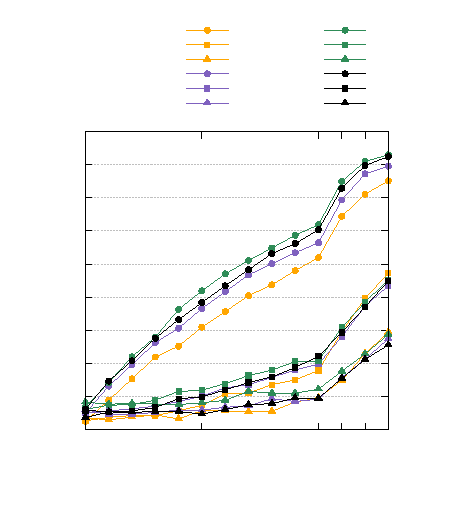
\includegraphics{../plots/strategies-acceptancerate}}%
    \gplfronttext
  \end{picture}%
\endgroup
